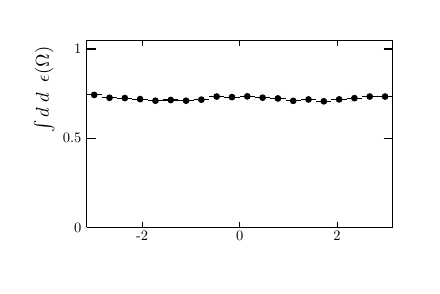
\begin{tikzpicture}
\pgfdeclareplotmark{cross} {
\pgfpathmoveto{\pgfpoint{-0.3\pgfplotmarksize}{\pgfplotmarksize}}
\pgfpathlineto{\pgfpoint{+0.3\pgfplotmarksize}{\pgfplotmarksize}}
\pgfpathlineto{\pgfpoint{+0.3\pgfplotmarksize}{0.3\pgfplotmarksize}}
\pgfpathlineto{\pgfpoint{+1\pgfplotmarksize}{0.3\pgfplotmarksize}}
\pgfpathlineto{\pgfpoint{+1\pgfplotmarksize}{-0.3\pgfplotmarksize}}
\pgfpathlineto{\pgfpoint{+0.3\pgfplotmarksize}{-0.3\pgfplotmarksize}}
\pgfpathlineto{\pgfpoint{+0.3\pgfplotmarksize}{-1.\pgfplotmarksize}}
\pgfpathlineto{\pgfpoint{-0.3\pgfplotmarksize}{-1.\pgfplotmarksize}}
\pgfpathlineto{\pgfpoint{-0.3\pgfplotmarksize}{-0.3\pgfplotmarksize}}
\pgfpathlineto{\pgfpoint{-1.\pgfplotmarksize}{-0.3\pgfplotmarksize}}
\pgfpathlineto{\pgfpoint{-1.\pgfplotmarksize}{0.3\pgfplotmarksize}}
\pgfpathlineto{\pgfpoint{-0.3\pgfplotmarksize}{0.3\pgfplotmarksize}}
\pgfpathclose
\pgfusepathqstroke
}
\pgfdeclareplotmark{cross*} {
\pgfpathmoveto{\pgfpoint{-0.3\pgfplotmarksize}{\pgfplotmarksize}}
\pgfpathlineto{\pgfpoint{+0.3\pgfplotmarksize}{\pgfplotmarksize}}
\pgfpathlineto{\pgfpoint{+0.3\pgfplotmarksize}{0.3\pgfplotmarksize}}
\pgfpathlineto{\pgfpoint{+1\pgfplotmarksize}{0.3\pgfplotmarksize}}
\pgfpathlineto{\pgfpoint{+1\pgfplotmarksize}{-0.3\pgfplotmarksize}}
\pgfpathlineto{\pgfpoint{+0.3\pgfplotmarksize}{-0.3\pgfplotmarksize}}
\pgfpathlineto{\pgfpoint{+0.3\pgfplotmarksize}{-1.\pgfplotmarksize}}
\pgfpathlineto{\pgfpoint{-0.3\pgfplotmarksize}{-1.\pgfplotmarksize}}
\pgfpathlineto{\pgfpoint{-0.3\pgfplotmarksize}{-0.3\pgfplotmarksize}}
\pgfpathlineto{\pgfpoint{-1.\pgfplotmarksize}{-0.3\pgfplotmarksize}}
\pgfpathlineto{\pgfpoint{-1.\pgfplotmarksize}{0.3\pgfplotmarksize}}
\pgfpathlineto{\pgfpoint{-0.3\pgfplotmarksize}{0.3\pgfplotmarksize}}
\pgfpathclose
\pgfusepathqfillstroke
}
\pgfdeclareplotmark{newstar} {
\pgfpathmoveto{\pgfqpoint{0pt}{\pgfplotmarksize}}
\pgfpathlineto{\pgfqpointpolar{44}{0.5\pgfplotmarksize}}
\pgfpathlineto{\pgfqpointpolar{18}{\pgfplotmarksize}}
\pgfpathlineto{\pgfqpointpolar{-20}{0.5\pgfplotmarksize}}
\pgfpathlineto{\pgfqpointpolar{-54}{\pgfplotmarksize}}
\pgfpathlineto{\pgfqpointpolar{-90}{0.5\pgfplotmarksize}}
\pgfpathlineto{\pgfqpointpolar{234}{\pgfplotmarksize}}
\pgfpathlineto{\pgfqpointpolar{198}{0.5\pgfplotmarksize}}
\pgfpathlineto{\pgfqpointpolar{162}{\pgfplotmarksize}}
\pgfpathlineto{\pgfqpointpolar{134}{0.5\pgfplotmarksize}}
\pgfpathclose
\pgfusepathqstroke
}
\pgfdeclareplotmark{newstar*} {
\pgfpathmoveto{\pgfqpoint{0pt}{\pgfplotmarksize}}
\pgfpathlineto{\pgfqpointpolar{44}{0.5\pgfplotmarksize}}
\pgfpathlineto{\pgfqpointpolar{18}{\pgfplotmarksize}}
\pgfpathlineto{\pgfqpointpolar{-20}{0.5\pgfplotmarksize}}
\pgfpathlineto{\pgfqpointpolar{-54}{\pgfplotmarksize}}
\pgfpathlineto{\pgfqpointpolar{-90}{0.5\pgfplotmarksize}}
\pgfpathlineto{\pgfqpointpolar{234}{\pgfplotmarksize}}
\pgfpathlineto{\pgfqpointpolar{198}{0.5\pgfplotmarksize}}
\pgfpathlineto{\pgfqpointpolar{162}{\pgfplotmarksize}}
\pgfpathlineto{\pgfqpointpolar{134}{0.5\pgfplotmarksize}}
\pgfpathclose
\pgfusepathqfillstroke
}
\definecolor{c}{rgb}{1,1,1};
\draw [color=c, fill=c] (0.1,0.0627517) rectangle (4.9,3.07483);
\draw [color=c, fill=c] (0.772,0.544685) rectangle (4.66,2.92423);
\definecolor{c}{rgb}{0,0,0};
\draw [c] (0.772,0.544685) -- (0.772,2.92423) -- (4.66,2.92423) -- (4.66,0.544685) -- (0.772,0.544685);
\draw [c,line width=0.4] (0.8692,2.2183) -- (0.8692,2.22803);
\draw [c,line width=0.4] (0.8692,2.22803) -- (0.8692,2.23776);
\draw [c,line width=0.4] (0.772,2.22803) -- (0.8692,2.22803);
\draw [c,line width=0.4] (0.8692,2.22803) -- (0.9664,2.22803);
\foreach \P in {(0.8692,2.22803)}{\draw[mark options={color=c,fill=c},mark size=2.402402pt,mark=*,mark size=1pt] plot coordinates {\P};}
\draw [c,line width=0.4] (1.0636,2.18198) -- (1.0636,2.19168);
\draw [c,line width=0.4] (1.0636,2.19168) -- (1.0636,2.20137);
\draw [c,line width=0.4] (0.9664,2.19168) -- (1.0636,2.19168);
\draw [c,line width=0.4] (1.0636,2.19168) -- (1.1608,2.19168);
\foreach \P in {(1.0636,2.19168)}{\draw[mark options={color=c,fill=c},mark size=2.402402pt,mark=*,mark size=1pt] plot coordinates {\P};}
\draw [c,line width=0.4] (1.258,2.17794) -- (1.258,2.18793);
\draw [c,line width=0.4] (1.258,2.18793) -- (1.258,2.19791);
\draw [c,line width=0.4] (1.1608,2.18793) -- (1.258,2.18793);
\draw [c,line width=0.4] (1.258,2.18793) -- (1.3552,2.18793);
\foreach \P in {(1.258,2.18793)}{\draw[mark options={color=c,fill=c},mark size=2.402402pt,mark=*,mark size=1pt] plot coordinates {\P};}
\draw [c,line width=0.4] (1.4524,2.16461) -- (1.4524,2.17474);
\draw [c,line width=0.4] (1.4524,2.17474) -- (1.4524,2.18486);
\draw [c,line width=0.4] (1.3552,2.17474) -- (1.4524,2.17474);
\draw [c,line width=0.4] (1.4524,2.17474) -- (1.5496,2.17474);
\foreach \P in {(1.4524,2.17474)}{\draw[mark options={color=c,fill=c},mark size=2.402402pt,mark=*,mark size=1pt] plot coordinates {\P};}
\draw [c,line width=0.4] (1.6468,2.14408) -- (1.6468,2.15428);
\draw [c,line width=0.4] (1.6468,2.15428) -- (1.6468,2.16448);
\draw [c,line width=0.4] (1.5496,2.15428) -- (1.6468,2.15428);
\draw [c,line width=0.4] (1.6468,2.15428) -- (1.744,2.15428);
\foreach \P in {(1.6468,2.15428)}{\draw[mark options={color=c,fill=c},mark size=2.402402pt,mark=*,mark size=1pt] plot coordinates {\P};}
\draw [c,line width=0.4] (1.8412,2.1529) -- (1.8412,2.16313);
\draw [c,line width=0.4] (1.8412,2.16313) -- (1.8412,2.17335);
\draw [c,line width=0.4] (1.744,2.16313) -- (1.8412,2.16313);
\draw [c,line width=0.4] (1.8412,2.16313) -- (1.9384,2.16313);
\foreach \P in {(1.8412,2.16313)}{\draw[mark options={color=c,fill=c},mark size=2.402402pt,mark=*,mark size=1pt] plot coordinates {\P};}
\draw [c,line width=0.4] (2.0356,2.14437) -- (2.0356,2.15449);
\draw [c,line width=0.4] (2.0356,2.15449) -- (2.0356,2.16461);
\draw [c,line width=0.4] (1.9384,2.15449) -- (2.0356,2.15449);
\draw [c,line width=0.4] (2.0356,2.15449) -- (2.1328,2.15449);
\foreach \P in {(2.0356,2.15449)}{\draw[mark options={color=c,fill=c},mark size=2.402402pt,mark=*,mark size=1pt] plot coordinates {\P};}
\draw [c,line width=0.4] (2.23,2.15789) -- (2.23,2.16774);
\draw [c,line width=0.4] (2.23,2.16774) -- (2.23,2.1776);
\draw [c,line width=0.4] (2.1328,2.16774) -- (2.23,2.16774);
\draw [c,line width=0.4] (2.23,2.16774) -- (2.3272,2.16774);
\foreach \P in {(2.23,2.16774)}{\draw[mark options={color=c,fill=c},mark size=2.402402pt,mark=*,mark size=1pt] plot coordinates {\P};}
\draw [c,line width=0.4] (2.4244,2.19739) -- (2.4244,2.2071);
\draw [c,line width=0.4] (2.4244,2.2071) -- (2.4244,2.2168);
\draw [c,line width=0.4] (2.3272,2.2071) -- (2.4244,2.2071);
\draw [c,line width=0.4] (2.4244,2.2071) -- (2.5216,2.2071);
\foreach \P in {(2.4244,2.2071)}{\draw[mark options={color=c,fill=c},mark size=2.402402pt,mark=*,mark size=1pt] plot coordinates {\P};}
\draw [c,line width=0.4] (2.6188,2.19035) -- (2.6188,2.19993);
\draw [c,line width=0.4] (2.6188,2.19993) -- (2.6188,2.20951);
\draw [c,line width=0.4] (2.5216,2.19993) -- (2.6188,2.19993);
\draw [c,line width=0.4] (2.6188,2.19993) -- (2.716,2.19993);
\foreach \P in {(2.6188,2.19993)}{\draw[mark options={color=c,fill=c},mark size=2.402402pt,mark=*,mark size=1pt] plot coordinates {\P};}
\draw [c,line width=0.4] (2.8132,2.20003) -- (2.8132,2.2096);
\draw [c,line width=0.4] (2.8132,2.2096) -- (2.8132,2.21917);
\draw [c,line width=0.4] (2.716,2.2096) -- (2.8132,2.2096);
\draw [c,line width=0.4] (2.8132,2.2096) -- (2.9104,2.2096);
\foreach \P in {(2.8132,2.2096)}{\draw[mark options={color=c,fill=c},mark size=2.402402pt,mark=*,mark size=1pt] plot coordinates {\P};}
\draw [c,line width=0.4] (3.0076,2.18314) -- (3.0076,2.19279);
\draw [c,line width=0.4] (3.0076,2.19279) -- (3.0076,2.20245);
\draw [c,line width=0.4] (2.9104,2.19279) -- (3.0076,2.19279);
\draw [c,line width=0.4] (3.0076,2.19279) -- (3.1048,2.19279);
\foreach \P in {(3.0076,2.19279)}{\draw[mark options={color=c,fill=c},mark size=2.402402pt,mark=*,mark size=1pt] plot coordinates {\P};}
\draw [c,line width=0.4] (3.202,2.17335) -- (3.202,2.18327);
\draw [c,line width=0.4] (3.202,2.18327) -- (3.202,2.1932);
\draw [c,line width=0.4] (3.1048,2.18327) -- (3.202,2.18327);
\draw [c,line width=0.4] (3.202,2.18327) -- (3.2992,2.18327);
\foreach \P in {(3.202,2.18327)}{\draw[mark options={color=c,fill=c},mark size=2.402402pt,mark=*,mark size=1pt] plot coordinates {\P};}
\draw [c,line width=0.4] (3.3964,2.14242) -- (3.3964,2.15247);
\draw [c,line width=0.4] (3.3964,2.15247) -- (3.3964,2.16252);
\draw [c,line width=0.4] (3.2992,2.15247) -- (3.3964,2.15247);
\draw [c,line width=0.4] (3.3964,2.15247) -- (3.4936,2.15247);
\foreach \P in {(3.3964,2.15247)}{\draw[mark options={color=c,fill=c},mark size=2.402402pt,mark=*,mark size=1pt] plot coordinates {\P};}
\draw [c,line width=0.4] (3.5908,2.16013) -- (3.5908,2.17054);
\draw [c,line width=0.4] (3.5908,2.17054) -- (3.5908,2.18095);
\draw [c,line width=0.4] (3.4936,2.17054) -- (3.5908,2.17054);
\draw [c,line width=0.4] (3.5908,2.17054) -- (3.688,2.17054);
\foreach \P in {(3.5908,2.17054)}{\draw[mark options={color=c,fill=c},mark size=2.402402pt,mark=*,mark size=1pt] plot coordinates {\P};}
\draw [c,line width=0.4] (3.7852,2.13658) -- (3.7852,2.14676);
\draw [c,line width=0.4] (3.7852,2.14676) -- (3.7852,2.15694);
\draw [c,line width=0.4] (3.688,2.14676) -- (3.7852,2.14676);
\draw [c,line width=0.4] (3.7852,2.14676) -- (3.8824,2.14676);
\foreach \P in {(3.7852,2.14676)}{\draw[mark options={color=c,fill=c},mark size=2.402402pt,mark=*,mark size=1pt] plot coordinates {\P};}
\draw [c,line width=0.4] (3.9796,2.1609) -- (3.9796,2.17108);
\draw [c,line width=0.4] (3.9796,2.17108) -- (3.9796,2.18125);
\draw [c,line width=0.4] (3.8824,2.17108) -- (3.9796,2.17108);
\draw [c,line width=0.4] (3.9796,2.17108) -- (4.0768,2.17108);
\foreach \P in {(3.9796,2.17108)}{\draw[mark options={color=c,fill=c},mark size=2.402402pt,mark=*,mark size=1pt] plot coordinates {\P};}
\draw [c,line width=0.4] (4.174,2.17674) -- (4.174,2.18684);
\draw [c,line width=0.4] (4.174,2.18684) -- (4.174,2.19694);
\draw [c,line width=0.4] (4.0768,2.18684) -- (4.174,2.18684);
\draw [c,line width=0.4] (4.174,2.18684) -- (4.2712,2.18684);
\foreach \P in {(4.174,2.18684)}{\draw[mark options={color=c,fill=c},mark size=2.402402pt,mark=*,mark size=1pt] plot coordinates {\P};}
\draw [c,line width=0.4] (4.3684,2.19752) -- (4.3684,2.20747);
\draw [c,line width=0.4] (4.3684,2.20747) -- (4.3684,2.21743);
\draw [c,line width=0.4] (4.2712,2.20747) -- (4.3684,2.20747);
\draw [c,line width=0.4] (4.3684,2.20747) -- (4.4656,2.20747);
\foreach \P in {(4.3684,2.20747)}{\draw[mark options={color=c,fill=c},mark size=2.402402pt,mark=*,mark size=1pt] plot coordinates {\P};}
\draw [c,line width=0.4] (4.5628,2.19745) -- (4.5628,2.20711);
\draw [c,line width=0.4] (4.5628,2.20711) -- (4.5628,2.21678);
\draw [c,line width=0.4] (4.4656,2.20711) -- (4.5628,2.20711);
\draw [c,line width=0.4] (4.5628,2.20711) -- (4.66,2.20711);
\foreach \P in {(4.5628,2.20711)}{\draw[mark options={color=c,fill=c},mark size=2.402402pt,mark=*,mark size=1pt] plot coordinates {\P};}
\draw [c,line width=0.4] (0.772,0.544685) -- (4.66,0.544685);
\draw [anchor= east] (4.66,0.207332) node[scale=0.672711, rotate=0]{$\phihel$};
\draw [c,line width=0.4] (1.47841,0.617878) -- (1.47841,0.544685);
\draw [c,line width=0.4] (2.716,0.617878) -- (2.716,0.544685);
\draw [c,line width=0.4] (3.95359,0.617878) -- (3.95359,0.544685);
\draw [c,line width=0.4] (1.47841,0.617878) -- (1.47841,0.544685);
\draw [c,line width=0.4] (3.95359,0.617878) -- (3.95359,0.544685);
\draw [anchor=base] (1.47841,0.382032) node[scale=0.52322, rotate=0]{-2};
\draw [anchor=base] (2.716,0.382032) node[scale=0.52322, rotate=0]{0};
\draw [anchor=base] (3.95359,0.382032) node[scale=0.52322, rotate=0]{2};
\draw [c,line width=0.4] (0.772,2.92423) -- (4.66,2.92423);
\draw [c,line width=0.4] (1.47841,2.85103) -- (1.47841,2.92423);
\draw [c,line width=0.4] (2.716,2.85103) -- (2.716,2.92423);
\draw [c,line width=0.4] (3.95359,2.85103) -- (3.95359,2.92423);
\draw [c,line width=0.4] (1.47841,2.85103) -- (1.47841,2.92423);
\draw [c,line width=0.4] (3.95359,2.85103) -- (3.95359,2.92423);
\draw [c,line width=0.4] (0.772,0.544685) -- (0.772,2.92423);
\draw [anchor= east] (0.2344,2.92423) node[scale=0.672711, rotate=90]{$\int d\thetaK \; d\thetamu \;\; \epsilon(\Omega) $};
\draw [c,line width=0.4] (0.88576,0.544685) -- (0.772,0.544685);
\draw [c,line width=0.4] (0.88576,1.6778) -- (0.772,1.6778);
\draw [c,line width=0.4] (0.88576,2.81092) -- (0.772,2.81092);
\draw [c,line width=0.4] (0.88576,2.81092) -- (0.772,2.81092);
\draw [anchor= east] (0.772,0.544685) node[scale=0.52322, rotate=0]{0};
\draw [anchor= east] (0.772,1.6778) node[scale=0.52322, rotate=0]{0.5};
\draw [anchor= east] (0.772,2.81092) node[scale=0.52322, rotate=0]{1};
\draw [c,line width=0.4] (4.66,0.544685) -- (4.66,2.92423);
\draw [c,line width=0.4] (4.54624,0.544685) -- (4.66,0.544685);
\draw [c,line width=0.4] (4.54624,1.6778) -- (4.66,1.6778);
\draw [c,line width=0.4] (4.54624,2.81092) -- (4.66,2.81092);
\draw [c,line width=0.4] (4.54624,2.81092) -- (4.66,2.81092);
\end{tikzpicture}
